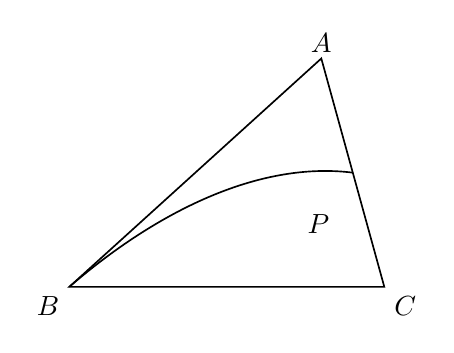
\begin{tikzpicture}[x=1cm,y=1cm,line width=.6pt,font=\normalsize]
\coordinate (B) at (0,0);
\coordinate (C) at (4,0);
\coordinate (T) at (3.2,2.9);
\coordinate (Q) at (3.60,1.45);
\draw (B)--(C)--(T)--cycle;
\draw (B) .. controls (1.1,0.95) and (2.4,1.6) .. (Q);
\node[below left] at (B) {$B$};
\node[below right] at (C) {$C$};
\node[right] at (2.9,0.80) {$P$};
\node[above,inner sep=2pt] at (T) {$A$};
\end{tikzpicture}
